\section{Einfach ungerade Dimension}
    Sei \(k\) ungerade und \(\mathcal{M}^{2k+1}\) eine \(\pi\)-Mannigfaltigkeit. Gem\"a\ss{} Satz \ref{lem:odd_dim_finite} kann angenommen werden, dass \(\mathcal{M}\) \((k-1)\)-zusammenh\"angend und \(H_k(\mathcal{M})\) endlich ist. Sei \(x\in H_k(\mathcal{M})\) und \(\mathcal{S}\) eine repr\"asentierende Sph\"are. Aus Dimensionsgr\"unden \ref{thm:vec_dim_triv} ist das Normalenb\"undel von \(\mathcal{S}\subseteq\mathring{\mathcal{M}}\) trivial, sodass Chirurgie an \(\mathcal{S}\) durchgef\"uhrt werden kann. Gem\"a\ss{} Satz \ref{thm:surg_framable} kann angenommen werden, dass eine derartige Chirurgie eine \(\pi\)-Mannigfaltigkeit ergibt. Das Problem in dieser Dimension besteht darin, dass eine derartige Chirurgie die Homologie nicht zwingenderma\ss en vereinfacht. Um dem beizukommen ist eine weitere sorgsame Reparametrisierung vonn\"oten. 

    \subsubsection{Effekt einer Reparametrisierung auf \(H_k(\mathcal{M}_0)\)}
        Seien \(\Phi\colon\mathbb{S}^k\times\mathbb{D}^{k+1}\hookrightarrow\mathring{\mathcal{M}}\) eine Anklebeeinbettung. Setze erneut \(\mathcal{D}:=\im\Phi\) und \({\mathcal{M}_0:=\mathcal{M}\setminus\mathring{\mathcal{D}}}\). Beachte, dass \({\partial\mathcal{D}\cong\mathbb{S}^k\times\mathbb{S}^k}\) gilt. Seien \(e,m\in H_k(\mathbb{S}^k\times\mathbb{S}^k)\) die Fundamentalklassen eines \"Aquators \({\mathbb{S}^k\times y}\) und eines Meridians \({x\times\mathbb{S}^k}\). Sei \(\gamma\colon\mathbb{S}^k\to\operatorname{SO}(k+1)\) glatt und 
        \[\Delta\colon\mathbb{S}^k\times\mathbb{S}^k\to\mathbb{S}^k\times\mathbb{S}^k,\,(x,y)\mapsto(x,\gamma(x)\cdot y)\]
        die zugeh\"orige Reparametrisierungsabbildung. Dann folgt aus dem Satz von Hurewicz, dass in \(H_k(\mathbb{S}^k\times\mathbb{S}^k)\) die Gleichungen
        \begin{equation}\label{eq:torus_reparam}
            e_0^{\gamma}:=\Delta_*e=e+\psi_*(\eqcl{\gamma})\,m\quad\text{und}\quad\Delta_*m=m\,.
        \end{equation}
        gelten. Es folgt, dass dies auch f\"ur \({e_0:=\phi_*e}\) und \(m_0:=\phi_*m\) in \(H_k(\mathcal{M}_0)\) gilt. Wie zuvor kann stets eine Reparametrisierung mit einem Element des Kernes der \(k\)-fach iterierten Einh\"angung \(S_*^k\) vorgenommen werden. Aus Stabilisierungsgr\"unden ist dies gerade die rechte Abbildung in dem Diagramm
        \begin{center}
            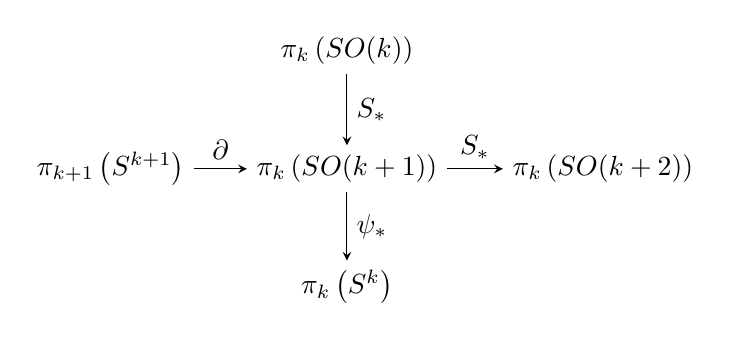
\begin{tikzpicture}
                \draw
                    (-3, 0) node (A) {\(\pi_{k+1}\left(\mathbb{S}^{k+1}\right)\)}
                    (0, 0) node (B) {\(\pi_k\left(\operatorname{SO}(k+1)\right)\)}
                    (3.25, 0) node (C) {\(\pi_k\left(\operatorname{SO}(k+2)\right)\)}
                    (0, 1.5) node (D) {\(\pi_k\left(\operatorname{SO}(k)\right)\)}
                    (0, -1.5) node (E) {\(\pi_k\left(\mathbb{S}^k\right)\)}
                    
                    (A) edge [-stealth] node [above] {\(\partial\)} (B)
                    (B) edge [-stealth] node [above] {\(S_*\)} (C)
                    
                    (D) edge [-stealth] node [right] {\(S_*\)} (B)
                    (B) edge [-stealth] node [right] {\(\psi_*\)} (E)
                    ;
            \end{tikzpicture}
        \end{center}
        Erneut wird \(\ker S_*\) wird von dem Tangentialb\"undel der Sph\"are erzeugt, und ist f\"ur gerade \(k\) zyklisch unendlich. Diese wird unter \(\psi_*\) auf das Doppelte eines Erzeugers abgebildet. Somit kann \(\psi_*\eqcl{\gamma}\) als jedes beliebige Vielfache von \(2\) gew\"ahlt werden.

    \subsubsection{Effekt einer Reparametrisierung auf den Rang von \(H_k(\mathcal{M}^{\prime})\)}
        Sei \(e^{\prime}\) das Bild von \(e_0\) in \(H_k(\mathcal{M})\) und \(m^{\prime}\) das Bild von \(m_0\) in \(H_k(\mathcal{M}^{\prime})\). Sei \(\ell\) der Rang von \(e^{\prime}\in H_k(\mathcal{M})\). Dann folgt aus der exakten Folge
        \[0\to\mathbb{Z}\xrightarrow{\lambda}H_k(\mathcal{M}_0)\to H_k(\mathcal{M})\to0\,,\]
        dass \(\ell e_0\in\im\lambda\) liegt. Dieses Bild besteht gerade aus den Vielfachen von \(m_0\), also existiert eine Abh\"angigkeit
        \[\ell e_0+\ell^{\prime}m_0=0\,.\]
        Wegen \(e_0^{\gamma}=e_0+\psi_*(\eqcl{\gamma})m_0\) folgt
        \[0=\ell e_0+\ell^{\prime}m_0=\ell\left(e_0^{\gamma}-\psi_*(\eqcl{\gamma})m_0\right)+\ell^{\prime}m_0=\ell e_0^{\gamma}-\left(\ell\psi_*(\eqcl{\gamma})+\ell^{\prime}\right)m_0\,.\]
        Folglich besitzt das Bild \(m_{\gamma}\) von \(m_0\) in \(\mathcal{M}_{\gamma}^{\prime}\) den Rang \(\abs{\ell\psi_*(\eqcl{\gamma})+\ell^{\prime}}\).
        Da weiterhin
        \[H_k\left(\mathcal{M}_{\gamma}^{\prime}\right)/\langle m_{\gamma}\rangle\cong H_k(\mathcal{M}_0)/\langle e_0,m_0\rangle\cong H_k\left(\mathcal{M}^{\prime}\right)/\langle m\rangle\]
        gilt, ist \(H_k\left(\mathcal{M}_{\gamma}^{\prime}\right)\) genau dann kleiner als \(H_k\left(\mathcal{M}\right)\), wenn 
        \[0<\abs{\ell\psi_*(\eqcl{\gamma})+\ell^{\prime}}\leq\ell\]
        ist. Da \(\eqcl{\gamma}\in\ker S_*\) so gew\"ahlt werden kann, dass \(\psi_*(\eqcl{\gamma})\) eine beliebige gerade Zahl ist, kann dies, insofern \(\ell^{\prime}\) nicht \(\ell\) teilt, stets m\"oglich. Um das Teilungsverhalten von \(\ell\) und \(\ell^{\prime}\) zu untersuchen wird die Verschlingungszahl ben\"otigt.

    \subsubsection{Verschlingungszahl}
        Sei \(\mathcal{M}^n\) eine orientierte Mannigfaltigkeit und \(n=i+j+1\). Die kurze exakte Folge von Kettenkomplexen
        \[0\to C_*\left(\mathcal{M};\mathbb{Z}\right)\mathop{\rightarrowtail}^pC_*\left(\mathcal{M};\mathbb{Q}\right)\twoheadrightarrow C_*\left(\mathcal{M};\mathbb{Q}/\mathbb{Z}\right)\to0\]
        induziert eine lange exakte Folge
        \[H_{i+1}\left(\mathcal{M};\mathbb{Q}/\mathbb{Z}\right)\xrightarrow{\partial}H_i\left(\mathcal{M};\mathbb{Z}\right)\xrightarrow{p_*}H_i\left(\mathcal{M};\mathbb{Q}\right)\to H_i\left(\mathcal{M};\mathbb{Q}/\mathbb{Z}\right)\]
        Seien \(x\in H_i(\mathcal{M})\) und \(y\in H_j(\mathcal{M})\) endlichen Ranges. Dann gilt \(p_*x=0\), sodass \(x\) zu einem \(\mu\in H_{i+1}(\mathcal{M};\mathbb{Q}/\mathbb{Z})\) mit \(\partial\mu=x\) zur\"uckgezogen werden kann. Definiere die Verschlingungszahl von \(x\) und \(y\) als Schnittzahl zweier repr\"a\-sen\-tie\-ren\-der Ketten mithilfe der Multiplikation \((\mathbb{Q}/\mathbb{Z})\times\mathbb{Z}\to\mathbb{Q}/\mathbb{Z}\). Die derart erhaltene Bilinearform ist nicht entartet, und es gilt
        \[L(x,y)+(-1)^{ij}L(y,x)\,.\]
        
        \begin{lemma}
            Sei \(k>1\) ungerade und \(\mathcal{M}^{2k+1}\) eine Mannigfaltigkeit, sodass \(H_k(\mathcal{M})\) endlich ist. Wird \(x\in H_k(\mathcal{M})\) vom Rang \(\ell\) durch Chirurgie an \(x\) durch ein Element vom Rang \(\ell^{\prime}\) ersetzt, gilt \(\ell/\ell^{\prime}=\pm L(x,x)\in\mathbb{Q}/\mathbb{Z}\).
        \end{lemma}
        \begin{proof}
            Sei \(z_1,z_2\in C_k(\mathcal{M}_0)\) Zyklen, die \(e_0\) und \(m_0\) repr\"asentieren. Wegen \(0=\ell e_0+\ell^{\prime}m_0\), existiert eine Kette \(c\in C_{k+1}(\mathcal{M}_0)\) mit
            \[\partial c=\ell z_1+\ell^{\prime}z_2\,.\]
            Sei \(c_1\in C_{k+1}(\mathcal{M})\) der durch \(\Phi(x\times\mathbb{D}^{k+1})\) definierte Zyklus mit \(\partial c_1=z_2\). Ist \(c_2\) jene durch \(\Phi(\mathbb{S}^k\times0)\) definierte Kette, die \(e\) repr\"asentiert, so gilt
            \[\partial(c-\ell^{\prime}c_1)/\ell=z_1\quad\text{und somit}\quad L(e,e)=(c-\ell^{\prime}c_1)/\ell\cdot c_2\,,\]
            Da \(c_2\) und \(c\) disjunkt sind gilt \(c\cdot c_2\) gleich null, und da \(c_1\) und \(c_2\) genau einen Schnittpunkt in \((x,0)\) besitzen gilt \(c_1\cdot c_2=\mp1\). Es folgt \(L(e,e)=\mp\ell^{\prime}/\ell\).
        \end{proof}
        \begin{corollary}\label{cor:link_nzero_small}
            Sei \(k>1\) ungerade und \(\mathcal{M}^{2k+1}\) eine \(\pi\)-Mannigfaltigkeit, sodass \(H_k(\mathcal{M})\) endlich ist. Existiert ein \(x\in H_k(\mathcal{M})\) mit \(L(x,x)\not=0\), kann \(H_k(\mathcal{M})\) durch eine gerahmte Chirurgie verkleinert werden. 
        \end{corollary}
        Auf diese Art und Weise kann \(H_k(\mathcal{M})\) so lange weiter verkleinert werden, bis keine \(x\) mit \(L(x,x)\not=0\) mehr existieren. Dann besitzt die Gruppe wegen folgendem Lemma jedoch eine besonders einfache Struktur.
        \begin{lemma}\label{lem:link_z2}
            Sei \(k>1\) ungerade und \(\mathcal{M}^{2k+1}\) eine Mannigfaltigkeit, sodass \(H_k(\mathcal{M})\) endlich ist. Gilt \(L(x,x)=0\) f\"ur alle \(x\in H_k(\mathcal{M})\), ist \(H_k(\mathcal{M})\cong(\mathbb{Z}_2)^s\).
        \end{lemma}
        \begin{proof}
            Aus \({L(\epsilon,\delta)+(-1)^{ij}L(\delta,\epsilon)=0}\) folgt, dass die Verschlingungspaarung f\"ur \({i=j}\) symmetrisch ist. Da \(L(x,x)=0\) f\"ur alle \(x\in H_k(\mathcal{M})\) gilt, ergibt sich
            \[0=L(\epsilon+\delta,\epsilon+\delta)=L(\epsilon,\epsilon)+2L(\epsilon,\delta)+L(\delta,\delta)=2L(\epsilon,\delta)\,.\]
            Da die Verschlingungspaarung nicht entartet ist, folgt aus \(L(2\epsilon,\delta)=0\) f\"ur alle \(\delta\) bereits \(2\epsilon=0\).
        \end{proof}

        \begin{lemma}\label{lem:rep_group}
            Sei \(k>1\) ungerade. Ist \(\mathcal{M}^{2k+1}\) eine geschlossene \((k-1)\)-zu\-sam\-men\-h\"an\-gen\-de \(\pi\)-Mannig\-faltig\-keit mit \(H_k(\mathcal{M})\cong(\mathbb{Z}_2)^s\), kann eine gerahmte Chirurgie an \(\mathcal{M}\) durchgef\"uhrt werden, sodass 
            \begin{equation}\label{eq:surg_poss}
                H_k(\mathcal{M}^{\prime})\cong\mathbb{Z}\oplus(\mathbb{Z}_2)^{s-2}\quad\text{oder}\quad H_k(\mathcal{M}^{\prime})\cong\mathbb{Z}_4\oplus(\mathbb{Z}_2)^{s-2}
            \end{equation}
            ist.
        \end{lemma}
        \begin{proof}
            Sei \(x\in H_k(\mathcal{M})\). Setze \({\mathcal{W}:=\mathcal{M}\times\mathbb{I}\multimap\mathbb{D}^{k+1}}\) und \({\mathcal{M}^{\prime}:=\mathcal{M}\multimap\mathbb{S}^k}\) sodass die Anklebesph\"are \(x\) repr\"asentiere. F\"ur das \(k\)-te Steenrod-Quadrat gilt
            \[\operatorname{Sq}^k\colon H^{k+1}(\mathcal{W},\partial\mathcal{W};\mathbb{F}_2)\to H^{2k+1}(\mathcal{W},\partial\mathcal{W};\mathbb{F}_2)\cong H_1(\mathcal{W};\mathbb{F}_2)=0\]
            sodass aus der Adem-Beziehung \({\operatorname{Sq}^{k+1}=\operatorname{Sq}^1\smile\operatorname{Sq}^k}\) bereits \(\operatorname{Sq}^{k+1}=0\) folgt. Dies zeigt f\"ur alle \(x\in H_{k+1}(\mathcal{W};\mathbb{F}_2)\) die Gleichung
            \[x\cdot x=\left\langle x^*\smile x^*,\eqcl{\mathcal{W}}\right\rangle=\big\langle\operatorname{Sq}^{k+1}(x^*),\eqcl{\mathcal{W}}\big\rangle=0\,,\]
            sodass die Schnittform auf \(H_{k+1}(\mathcal{W};\mathbb{F}_2)\) geraden Rang besitzt. Gem\"a\ss{} Lemma \ref{lem:srg_chg_field_betti} folgt, dass \(\dim_{\mathbb{F}_2}H_k(\mathcal{M}^{\prime};\mathbb{F}_2)\not=\dim_{\mathbb{F}_2}H_k(\mathcal{M};\mathbb{F}_2)\) gilt. Eine Chirurgie kann wie zuvor so reparametrisiert werden, dass \(x\) durch ein Element \(x^{\prime}\in H_k(\mathcal{M}^{\prime})\) geraden Ranges \(\ell^{\prime}\) mit \(0\leq\ell^{\prime}\leq2\) ersetzt wird. Somit ist \(\ell^{\prime}\) entweder null oder zwei. Aus
            \[H_k(\mathcal{M}^{\prime})/\langle x^{\prime}\rangle\cong H_k(\mathcal{M})/\langle x\rangle\cong(\mathbb{Z}_2)^{s-1}\]
            folgt die Existenz einer kurzen exakten Folge
            \[0\to\mathbb{Z}_{\ell^{\prime}}\rightarrowtail H_k(\mathcal{M}^{\prime})\twoheadrightarrow(\mathbb{Z}_2)^{s-1}\to0\,.\]
            Beachte \(\mathbb{Z}_0=\mathbb{Z}/0\mathbb{Z}\cong\mathbb{Z}\). W\"urde diese spalten, g\"olte \(H_k(\mathcal{M}^{\prime};\mathbb{F}_2)\cong\mathbb{Z}_2\oplus(\mathbb{Z}_2)^{s-1}\), was ein Widerspruch gegen den Fakt w\"are, dass die Chirurgie die \(\mathbb{F}_2\)-Dimension ver\"andert. Folglich bleiben lediglich die M\"og\-lich\-kei\-ten aus Gleichung \ref{eq:surg_poss}.
        \end{proof}

        \begin{lemma}\label{lem:link_zero_small}
            Sei \(k>1\) ungerade und \(\mathcal{M}^{2k+1}\) eine \((k-1)\)-zu\-sam\-men\-h\"an\-gen\-de \(\pi\)-Mannigfaltigkeit, deren Rand leer oder eine Homotopiesph\"are ist sodass \(H_k(\mathcal{M})\) endlich ist. Existiert \textbf{kein} \(x\in H_k(\mathcal{M})\) mit \(L(x,x)\not=0\), kann \(H_k(\mathcal{M})\) trotzdem durch eine gerahmte Chirurgie verkleinert werden.
        \end{lemma}
        \begin{proof}
            Da \(L(x,x)=0\) f\"ur alle \(x\in H_k(\mathcal{M})\) gilt, folgt aus Lemma \ref{lem:link_z2} \(H_k(\mathcal{M})\cong(\mathbb{Z}_2)^s\). Dann ist 
            \[\mathcal{N}:=\mathcal{M}\mathop{+}^{\partial\mathcal{M}}\mathcal{M}\quad\text{mit}\quad{H_k(\mathcal{N})}\cong H_k(\mathcal{M})\oplus H_k(\mathcal{M})\cong(\mathbb{Z}_2)^{2s}\]
            eine geschlossene Mannigfaltigkeit. Gem\"a\ss{} Lemma \ref{lem:rep_group} kann an \(\mathcal{N}\) eine Chirurgie durchgef\"uhrt werden, sodass 
            \[(\mathbb{Z}_2)^s\oplus H_k(\mathcal{M}\multimap\mathbb{S}^k)\cong H_k(\mathcal{N}\multimap\mathbb{S}^k)\cong(\mathbb{Z}_2)^s\oplus\begin{cases}
                \mathbb{Z}\oplus(\mathbb{Z}_2)^{s-2}\\
                \mathbb{Z}_4\oplus(\mathbb{Z}_2)^{s-1}
            \end{cases}\]
            gilt. Da \((\mathbb{Z}_2)^s\) gek\"urzt werden kann, ist \(H_k(\mathcal{M}\multimap\mathbb{S}^k)\) entweder zu \(\mathbb{Z}_4\oplus(\mathbb{Z}_2)^{s-1}\) oder zu \(\mathbb{Z}\oplus(\mathbb{Z}_2)^{s-2}\) isomorph. Im ersten Fall ergibt dies direkt eine kleinere Gruppe als \(H_k(\mathcal{M})\), im zweiten Fall muss vorher der direkte \(\mathbb{Z}\)-Summand mithilfe von Lemma \ref{lem:odd_dim_finite} eliminiert werden. 
        \end{proof}
        Aus Korollar \ref{cor:link_nzero_small} und Lemma \ref{lem:link_zero_small} folgt zusammen:
        \begin{corollary}\label{cor:single_odd_zero}
            Es gilt \(P^{4m+3}=0\).
        \end{corollary}